\documentclass[unicode, 14pt, aspectratio=169]{beamer}
\usepackage{bussproofs}
\usepackage{listings}
\usetheme{titechen}
\addbibresource{main.bib}
 \date{\today}
\title{The Origins of Type Theory}
\author{\texttt{ryotaro612}}
\newcommand\blfootnote[1]{%
  \begingroup
  \renewcommand\thefootnote{}\footnote{#1}%
  \addtocounter{footnote}{-1}%
  \endgroup
}

\begin{document}
\begin{frame}[noframenumbering, plain]
\titlepage
\end{frame}
\section{Introduction}
\begin{frame}
  \frametitle{Objective}
  {\large Introduction to fields related to the theory of types}
  \par
  \vspace{16pt}
  Fields related to the references of this slides
  \begin{itemize}
  \item Logic
  \item Set theory
  \item Semiotics
  \item Structuralism
  \item Philosophy of language
  \end{itemize}
\end{frame}
\section{Non-euclidean geometry}
\begin{frame}
  \frametitle{Geometry in ancient Greece}
  {\large The approach to develop Geometry in ancient Greece was deductive reasoning.}
\begin{columns}
  \begin{column}{0.25\textwidth}
    \begin{center}
      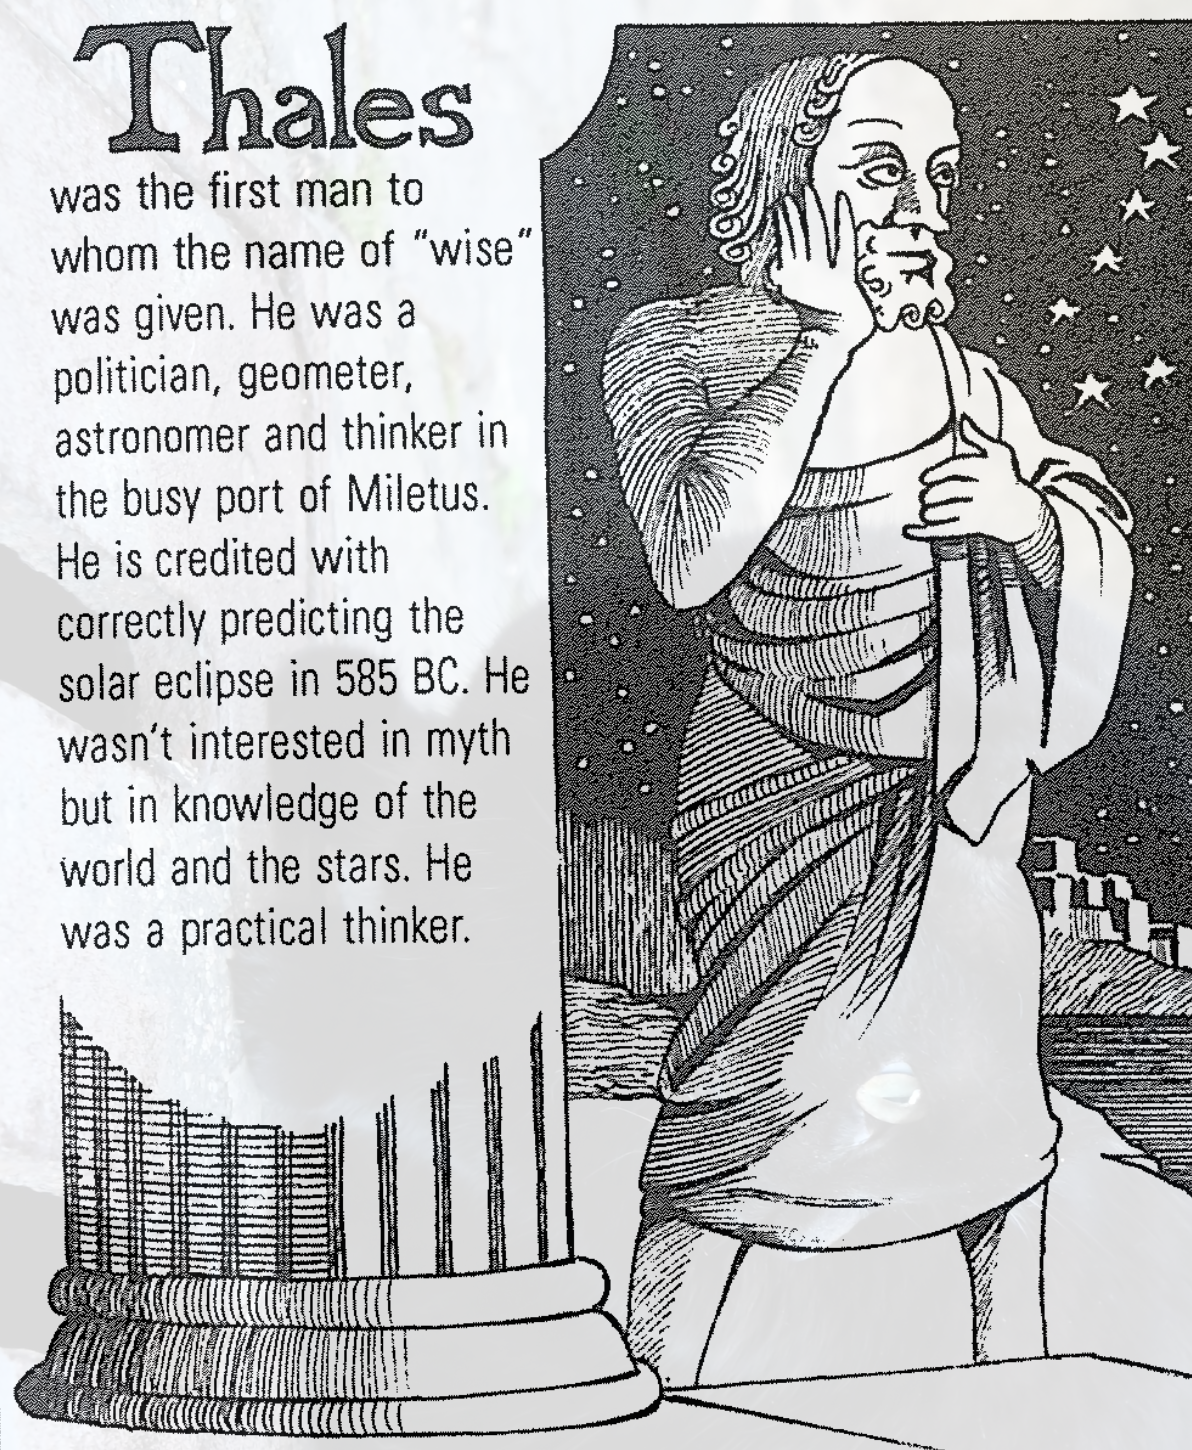
\includegraphics[width=0.7\textwidth]{images/thales.png}
    \end{center}
  \end{column}
  \begin{column}{0.25\textwidth}
    \begin{center}
      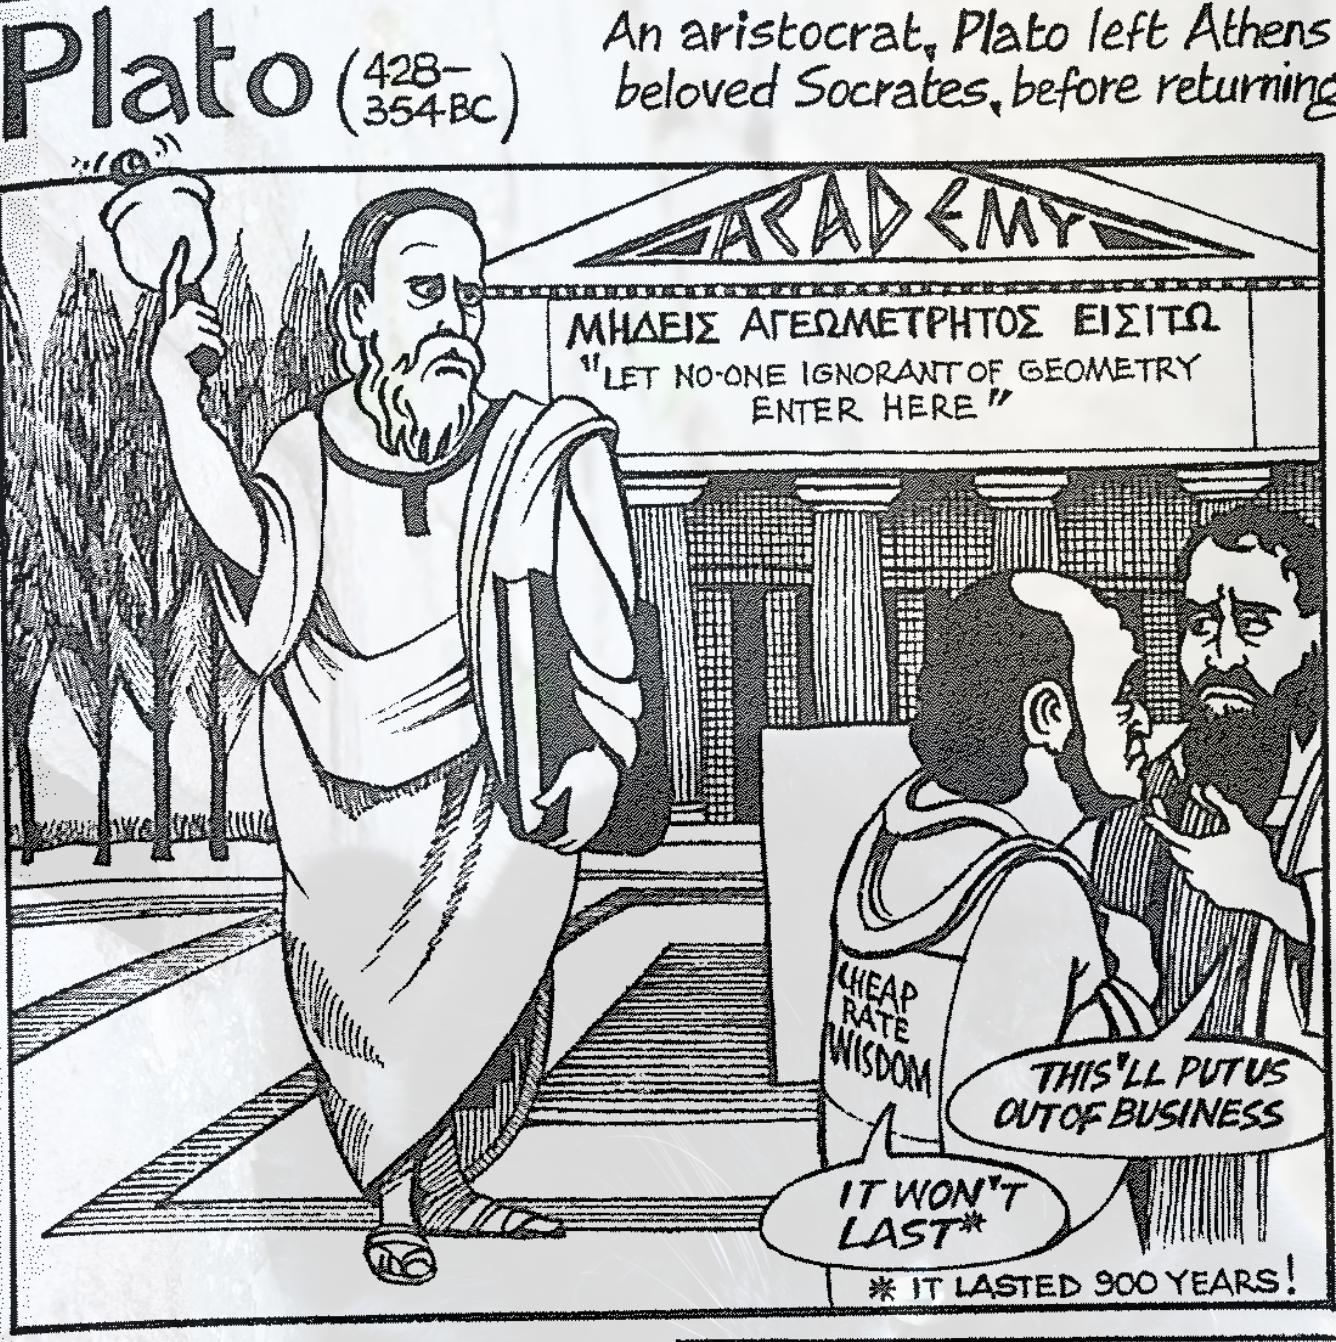
\includegraphics[width=0.7\textwidth]{images/plato.png}
    \end{center}
  \end{column}
  \begin{column}{0.25\textwidth}
    \begin{center}
      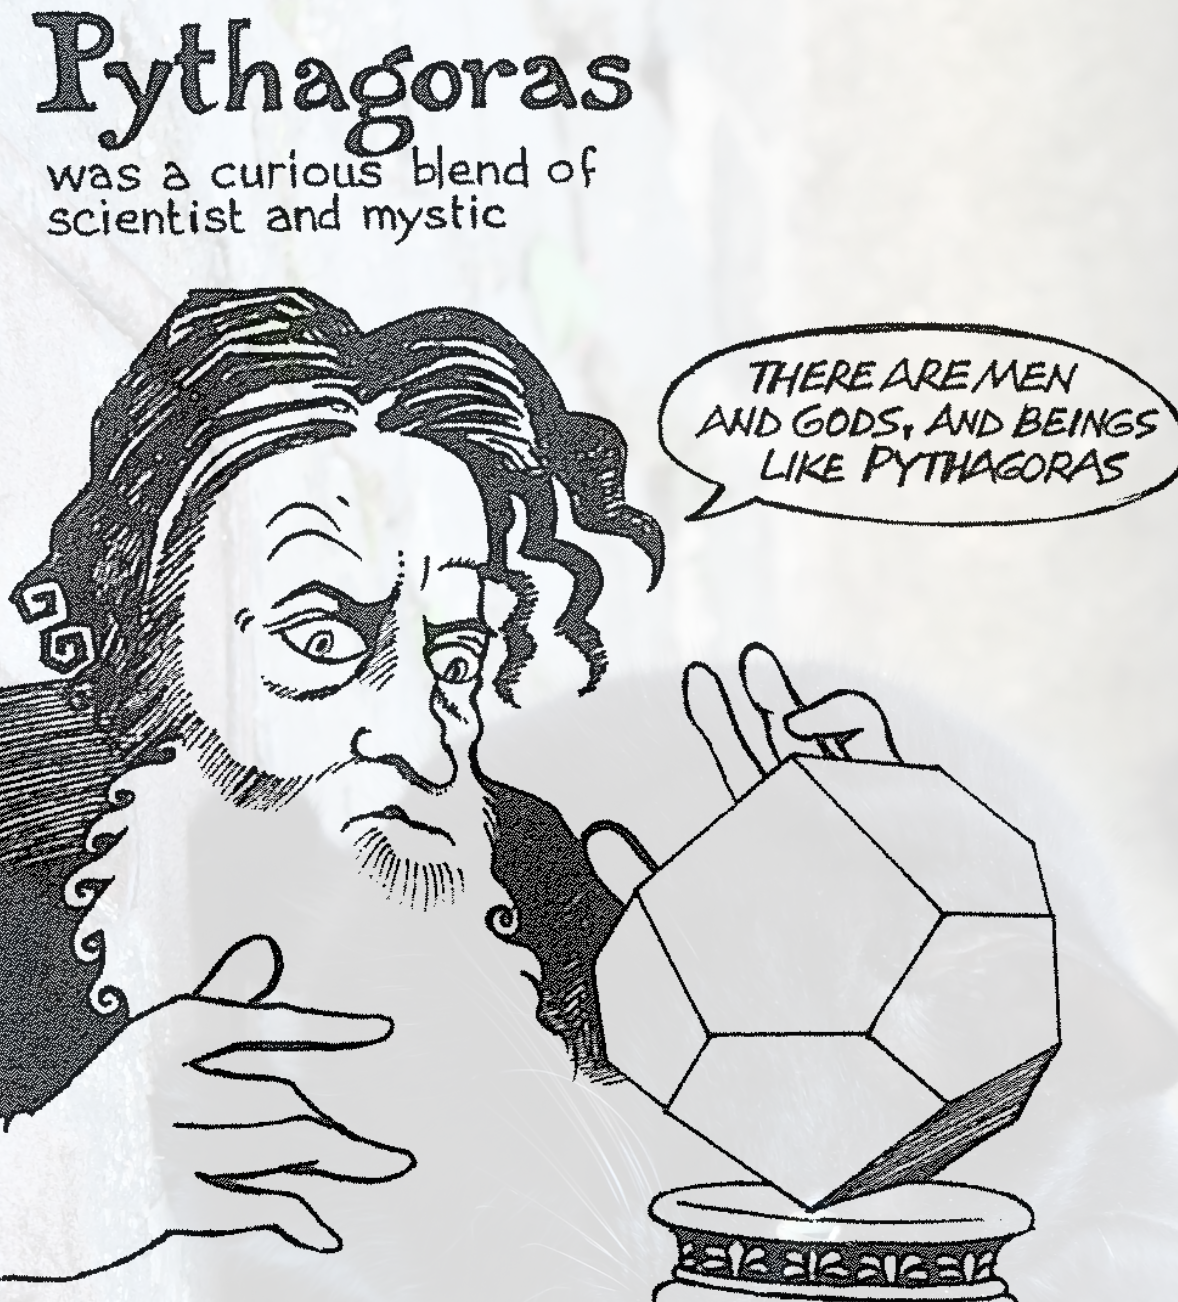
\includegraphics[width=0.7\textwidth]{images/pythagoras.png}
    \end{center}
  \end{column}
  \begin{column}{0.25\textwidth}
    \begin{center}
      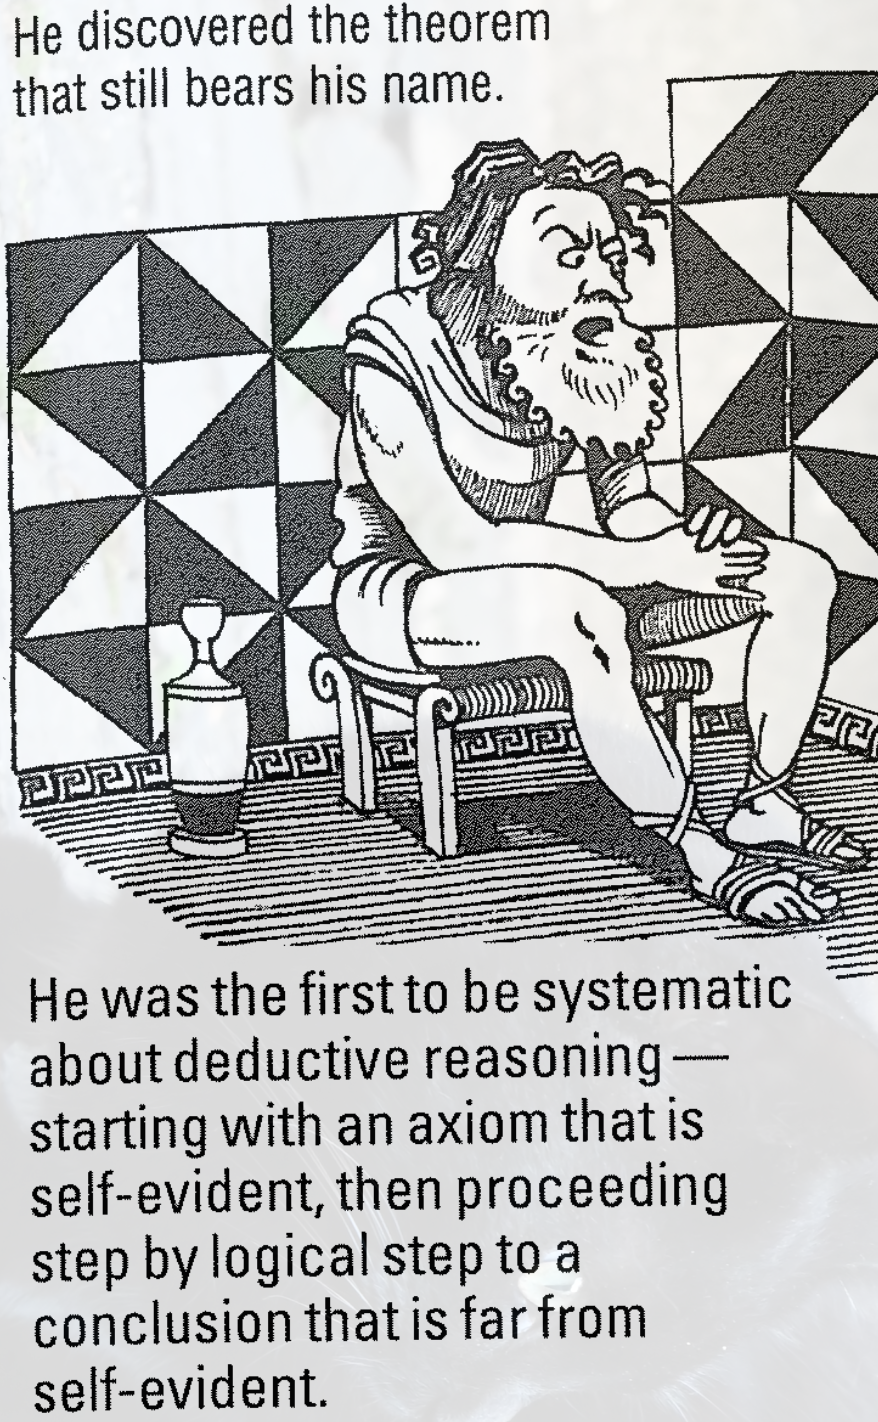
\includegraphics[width=0.7\textwidth]{images/pythagoras2.png}
    \end{center}
  \end{column}  
\end{columns}
\blfootnote{Images adapted from Philosophy for beginners\supercite{philosophy-for-begginers}}
\end{frame}
\begin{frame}
  \frametitle{Euclid's Elements}
  {\large Euclid's Elements is a collection of axioms, postulates, propositions, and proofs.}
  \par
  \vspace{16pt}
  \begin{description}[leftmargin=0cm]
  \item[Definition 1] A point is that of which there is no part.
  \item[Definition 2] A line is a length without breadth.
  \item[Definition 3] A surface is that which has length and breadth only.
  \item[Axiom 5] \textcolor{highlight}{The whole is greater than the part.}
  % \item[Proposition 5] For isosceles triangles, the angles at the base are equal to one another, and if the equal sides are produced then the angles under the base will be equal to one another.
  \end{description}
\end{frame}
\begin{frame}
  \frametitle{Euclid's postulates}
  {\large The fifth postulate never seemed self-evident.}
  \par
  {\footnotesize
  \begin{enumerate}
  \item Let it have been postulated to draw a straight-line from any point to any point.
  \item To produce a finite straight line continuously in a straight line.
  \item To draw a circle with any center and radius.
  \item All right-angles are equal to one another.
  \item If a straight-line falling across two straight-lines makes internal angles on the same side less than two right-angles, then the two (other) straight-lines, being produced to infinity meet on that side (of the original straight-line) that the (sum of the internal angles) is less than two right-angles (and do not meet on the other side).
  \end{enumerate}
  }
\end{frame}
\begin{frame}
  \frametitle{The fifth postulate is known as the parallel postulate.}
  {\large Given a straight line and a point not on that line, there is exactly one straight line parallel to the original line that passes through the given point.}
  \blfootnote{Figure adapted from 「数学の世界史」\supercite{suugaku-no-sekaishi}}
  \begin{figure}
    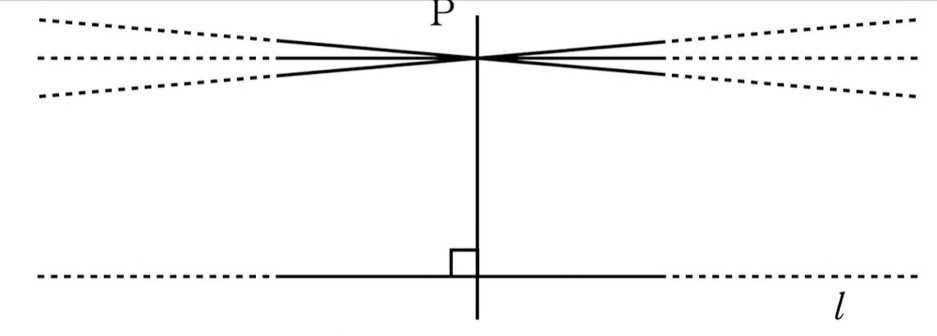
\includegraphics[width=0.6\textwidth]{images/axiom5.png}
    \caption{A parallel line and a point $p$ not on that line}
  \end{figure}
\end{frame}
\begin{frame}
  \frametitle{Investigations of the parallel postulate}
  \begin{itemize}
  \item Many attempts were made to derive the parallel postulate using the rest of the other postulates.
    \begin{itemize}
    \item Investigations were made by Alhazen (965-1039) and Khayyam (1048–1131).
    \item The Saccheri-Legendre Theorem states that if the parallel postulate is not assumed, then the sum of the angles of a triangle is less than or equal to 180 degrees.
    \end{itemize}
  \item The negation of the parallel postulate leads to no contradiction with the other postulates.
    \begin{itemize}
      \item Lobachevsky, along with János Bolyai, independently proposed a system where infinitely many parallels exist, leading to no contradictions within the geometry itself.
    \end{itemize}
  \end{itemize}
\end{frame}
\begin{frame}
  \frametitle{Examples of Non-Euclidean Spaces}
  {\large Great circles on a sphere must intersect.}
  \blfootnote{Figure from "An Introduction to Structuralism"\supercite{structure}}
  \begin{figure}
    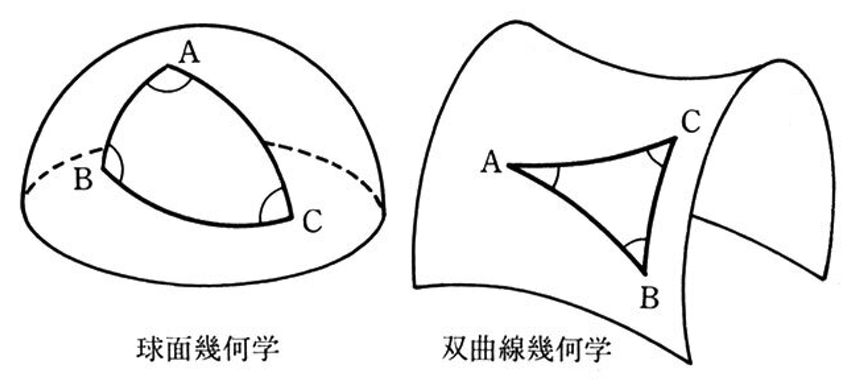
\includegraphics[width=0.5\textwidth]{images/non-euclid.png}
    \caption{Example of a non-Euclidean space}
  \end{figure}
  \begin{itemize}
  \item Great circles are cross-sections of spheres passing through the center.
  \item Great circles correspond to straight lines in Euclidean geometry.
  \end{itemize}
\end{frame}
% \section{Naive Set Theory}
% \begin{frame}
%   \frametitle{Impact of Non-Euclidean Geometry}
%   {\large Correctness is based on the axioms assumed.}
%   \begin{itemize}
%   \item Mathematical objects, including space, are constructed from axioms.
%     \begin{itemize}
%     \item Euclidean geometry feels correct because it aligns with naive visual experience.
%     \item Definitions of lines and planes in "Elements" are vague.
%     \end{itemize}
%   \item \textcolor{highlight}{Set theory} was established by Dedekind and Cantor as a tool to define mathematical objects.
%   \end{itemize}
% \end{frame}
% \begin{frame}
%   \frametitle{Thinking of Mathematics as Collections of Objects}
%   {\large Everything can be defined using the empty set.}
%   \par
%   Example
%   \begin{enumerate}
%   \item Define the empty set $\phi$ as $\{x|x\neq x\}$.
%   \item Name $\phi$ as $0$.
%   \item The set containing a single empty set $\{\phi\}$ is named $1$.
%   \item Name $\{0, 1\}$ as $2$.
%   \item $\vdots$
%   \item Name $\{0, 1, 2, \cdots\}$ as $\omega$.
%   \item Make the power set of $\omega$, $P(\omega)$, the set of real numbers.
%   \item Make $P(P(\omega))$ the set of functions from real numbers to real numbers.
%   \end{enumerate}
% \end{frame}
% \section{Symbolic Logic}
% \begin{frame}
%   \frametitle{Foundation of Arithmetic}
%   {\large Frege attempted to base arithmetic on logic.}
%   \begin{columns}
%     \begin{column}{0.8\textwidth}
%       \begin{itemize}
%       \item Proposed \textcolor{highlight}{predicate logic} in "Conceptual Notation."
%       \item Suggested axioms and theorems of arithmetic via conceptual notation and set theory in "The Basic Laws of Arithmetic."
%       \item In "On Sense and Reference," posited that words have both a sense and a reference.
%         \begin{itemize}
%         \item The reference of the "morning star" and "evening star" is Venus.
%         \item The sense of "Venus is the morning star" differs from "Venus is Venus."
%         \end{itemize}
%       \end{itemize}
%     \end{column}    
%     \begin{column}{0.2\textwidth}
%       \begin{figure}
%         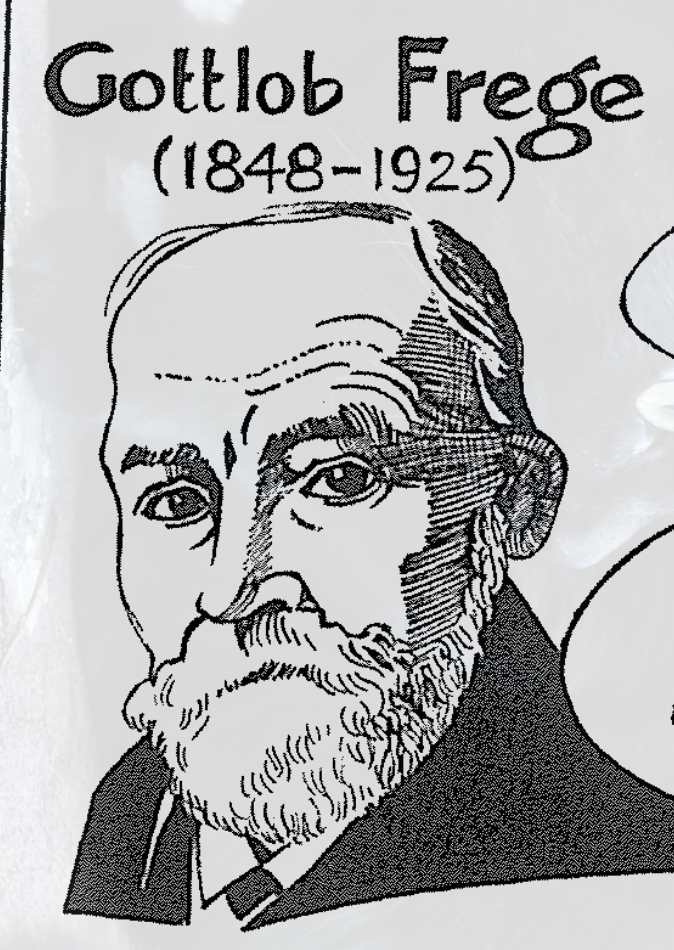
\includegraphics[width=1\textwidth]{images/frege.png}
%       \end{figure}       
%     \end{column} 
%   \end{columns}
%   \blfootnote{Figures from Philosophy for beginners\supercite{philosophy-for-begginers}}
% \end{frame}
% \begin{frame}
%   \frametitle{Formalizing Thought with Symbols}
%   {\large The idea to reduce inference to symbolic manipulation has existed since the 17th century or earlier.}  
%   \begin{columns}
%     \begin{column}{0.55\textwidth}
%       Those who devised it:
%       \begin{itemize}
%         \item Notation for calculus used today
%         \item The binary number system
%         \item \textcolor{highlight}{characteristica universalis}
%           \begin{itemize}
%           \item A set of symbols for thought analogous to the alphabet for language.
%           \item Reasoning is done through algebraic operations with symbols.
%           \end{itemize}
%       \end{itemize}
%     \end{column}    
%     \begin{column}{0.4\textwidth}
%       \begin{figure}
%         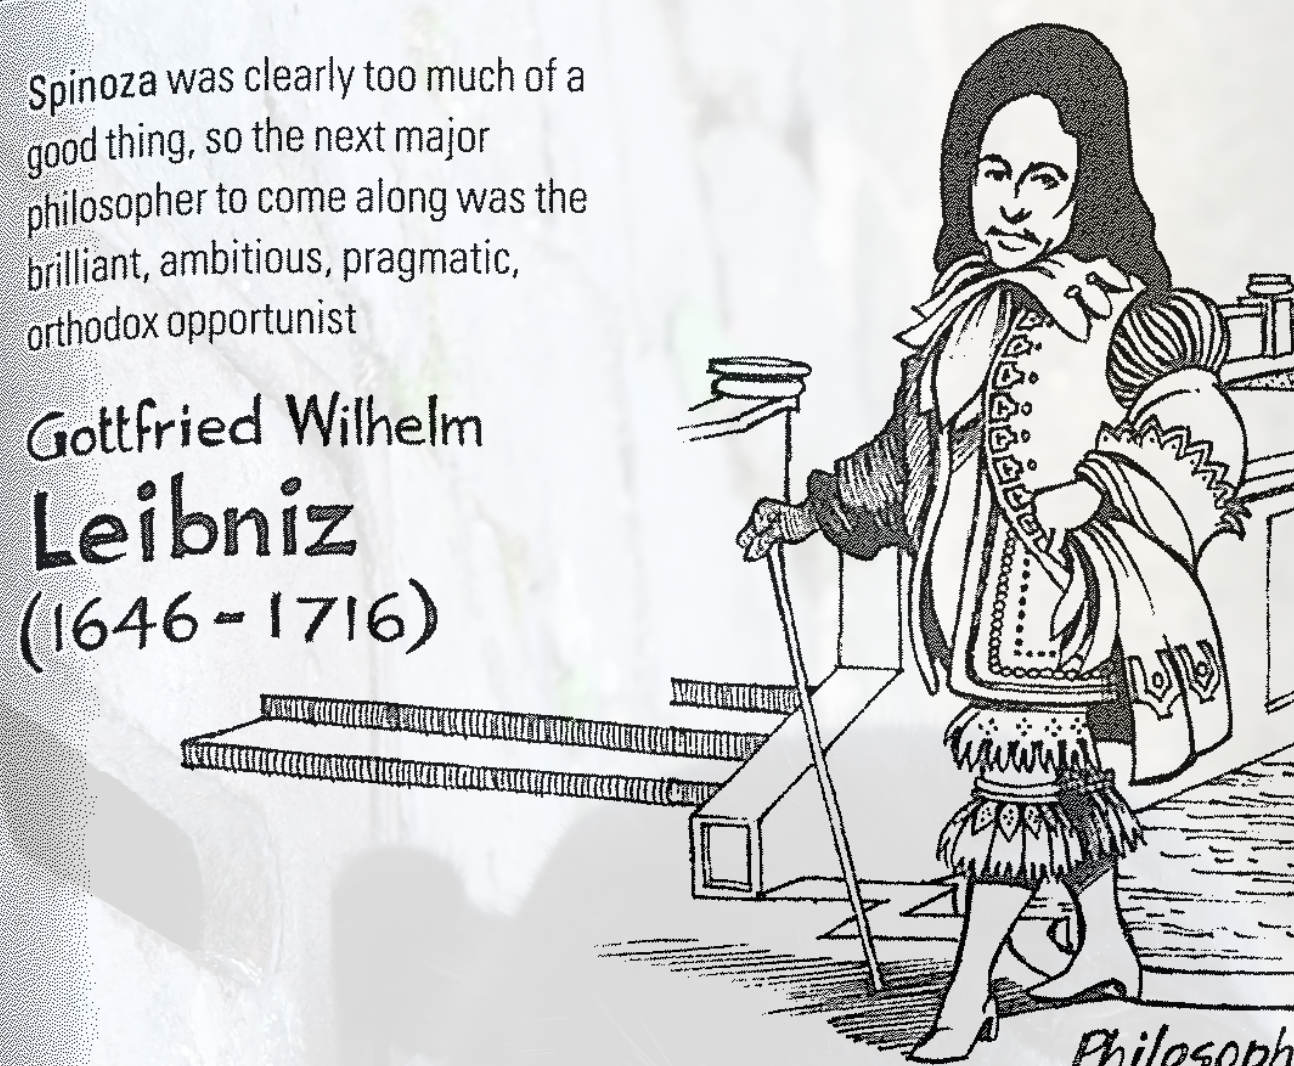
\includegraphics[width=0.7\linewidth]{images/leibniz.png}
%         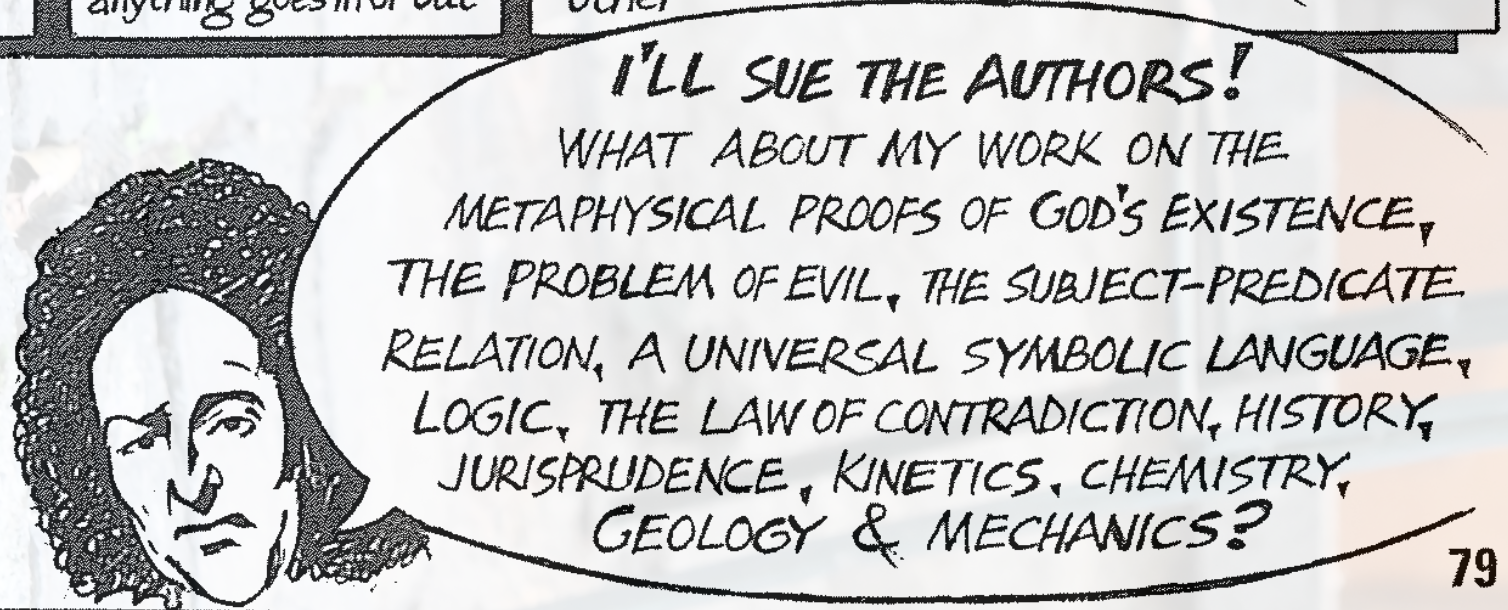
\includegraphics[width=0.7\linewidth]{images/universal.png}
%       \end{figure}       
%     \end{column} 
%   \end{columns}
%   \blfootnote{Figures from Philosophy for beginners\supercite{philosophy-for-begginers}}  
% \end{frame}
% \begin{frame}
%   \frametitle{Boole's Logical Algebra}
%   {\large Boole represented the sets of individuals appearing in propositions using symbols.}
%   \begin{columns}
%     \begin{column}{0.7\textwidth}
%       \begin{center}
%         Quotation from "The Laws of Thought"\supercite{bool}:
%         \begin{quotation}
%           Let us then agree to represent \textcolor{highlight}{the class of individuals to which a particular name or description is applicable, by a single letter, as x}. If the name is “men,” for instance, let x represent “all men,”
%         \end{quotation}
%       \end{center}
%     \end{column}    
%     \begin{column}{0.2\textwidth}
%       \begin{figure}
%         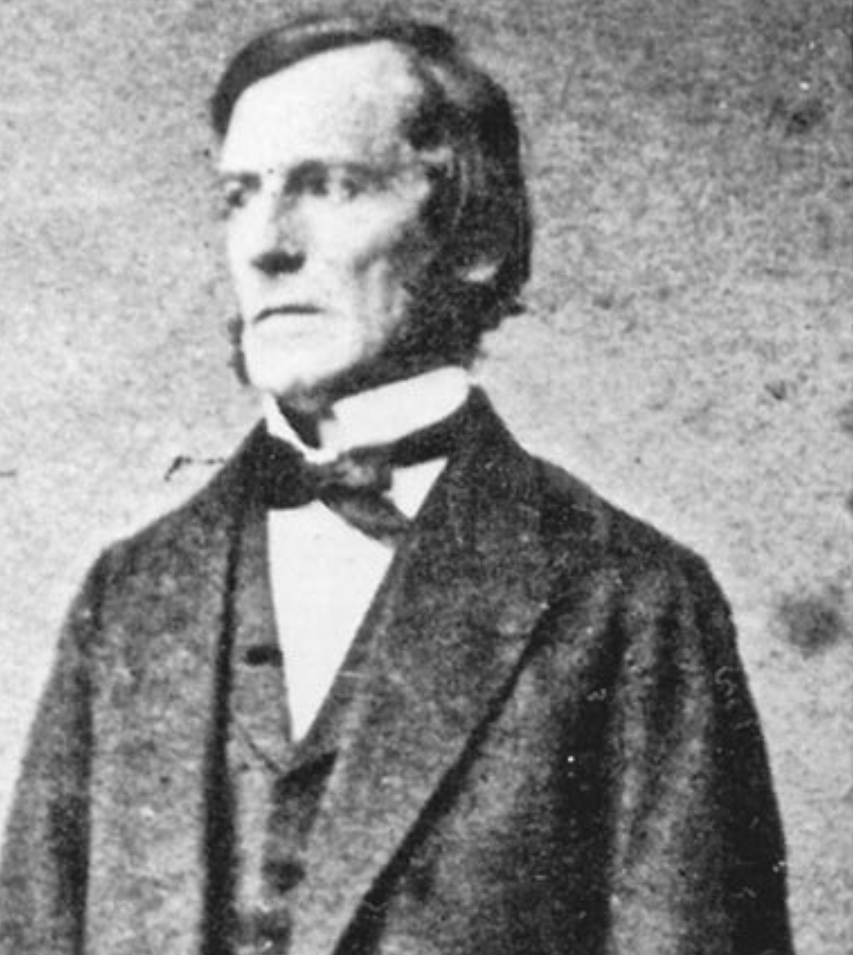
\includegraphics[width=1\textwidth]{images/bool.png}
%       \end{figure}       
%     \end{column} 
%   \end{columns}
%   \blfootnote{Figures from "The Universal Computer: The Road from Leibniz to Turing"}
% \end{frame}
% \begin{frame}
%   \frametitle{Examples of Inference Rules}
%   {\large Propositional logic is a logical system composed of propositions and logical connectives.}
%   \par
%   Inference rules:
%   \par
%   \vspace{16pt}
%   \AxiomC{$\varphi, \psi$}
%   \RightLabel{(\wedge Introduction)}
%   \UnaryInfC{$\varphi\wedge\psi$}
%   \DisplayProof
%   \AxiomC{$\varphi\wedge\psi$}
%   \RightLabel{(\vee Elimination)}
%   \UnaryInfC{$\varphi$}
%   \DisplayProof
%   \AxiomC{$\varphi\wedge\psi$}
%   \RightLabel{(\vee Elimination)}
%   \UnaryInfC{$\psi$}
%   \DisplayProof
%   \AxiomC{$[\varphi]$}
%   \noLine
%   \UnaryInfC{$\vdots$}
%   \noLine
%   \UnaryInfC{$\psi$}
%   \RightLabel{(\rightarrow Introduction)}  
%   \UnaryInfC{$\varphi\rightarrow\psi$}
%   \DisplayProof
%   \AxiomC{$\varphi$}
%   \AxiomC{$\varphi\rightarrow\psi$}
%   \RightLabel{(\rightarrow Elimination)}  
%   \BinaryInfC{$\psi$}
%   \DisplayProof
%   \AxiomC{$\bot$}
%   \RightLabel{($\bot$)}
%   \UnaryInfC{$\varphi$}
%   \DisplayProof
%   \AxiomC{$[\neg\varphi]$}
%   \noLine
%   \UnaryInfC{$\vdots$}
%   \noLine
%   \UnaryInfC{$\bot$}
%   \RightLabel{(Reductio ad Absurdum)}
%   \UnaryInfC{$\varphi$}
%   \DisplayProof
%   \par
%   $\varphi$, and $\psi$ are propositions that can take truth values.
% \end{frame}
% \begin{frame}
%   \frametitle{Conceptual Notation}
%   {\large Frege formalized statements with predicates.}
%   \begin{itemize}
%   \item Statements like “$\varphi$ is ~” are represented by predicates $P(\varphi)$ that map argument $\varphi$ to truth values, added to propositional logic.
%   \item \textcolor{highlight}{Also adds the universal quantifier $\forall$ for “for any $\phi$,” and the existential quantifier $\exists$ for “there exists $x$.”}
%   \item For instance, the statement “Pets at home are either dogs or cats” is represented as $\forall x. P(x) \rightarrow D(x) \vee C(x)$.
%   \item Complex propositions can be easily expressed as combinations of simpler ones.
%   \end{itemize} 
% \end{frame}
% \begin{frame}
%   \frametitle{Russell's Paradox}
%   {\large A contradiction arises when considering \textcolor{highlight}{sets of sets}.}
%   \begin{enumerate}
%   \item Define the set $R$ of all sets that do not contain themselves as a member: $R = \{x | x \notin x \}$.
%   \item If $R$ is a set that does not contain itself, then by definition, $R$ should be a member of $R$.
%   \item If $R$ is a set that contains itself, then by definition, $R$ should not be a member of $R$.
%   \end{enumerate}  
% \end{frame}
% \begin{frame}
%   \frametitle{Russell's Paradox in "The Basic Laws of Arithmetic"}
%   {\large The cause is Axiom V: \textcolor{highlight}{$\epsilon P = \epsilon Q \equiv \forall x [P(x) \equiv Q(x)]$.}}
%   \begin{itemize}
%   \item Axiom V is the condition for the identity of predicates.
%   \item $\epsilon P$ is the set fulfilling predicate $P$. 
%     \begin{enumerate}
%     \item $R$ can be expressed using predicate logic as $\exists P [x = \epsilon P \wedge \neg P(x)]$.
%     \item Substituting $x$ as $\epsilon R$, we obtain $R(\epsilon R) \equiv \neg R(\epsilon R)$.
%     \end{enumerate}
%   \item The beginning of type theory involved Russell's attempt to resolve the paradox by imposing a hierarchical structure, such as predicates of predicate logic not being able to take predicates.
%   \end{itemize}
% \end{frame}
\begin{frame}[allowframebreaks,t]
  \frametitle{References}
  \printbibliography
  \nocite{*}
\end{frame}

\end{document}
